\section{Bootstrapping Narrowband Photo-z}\label{sec:bootstrapping}
We use deep multiband redshift distributions as probabilistic training labels.
Here, ``narrowband'' refers to the full COSMOS photometry, including its
intermediate and narrow bands. ``Bootstrapping'' denotes transferring this
redshift information to broadband measurements; it is distinct from the
bootstrap resampling used to estimate statistical errors below.

Figure~\ref{fig:workflow} summarizes training. Deep multiband
redshift PDFs are needed only during training; inference uses broadband
fluxes and their uncertainties.

\begin{figure*}[t]
\centering
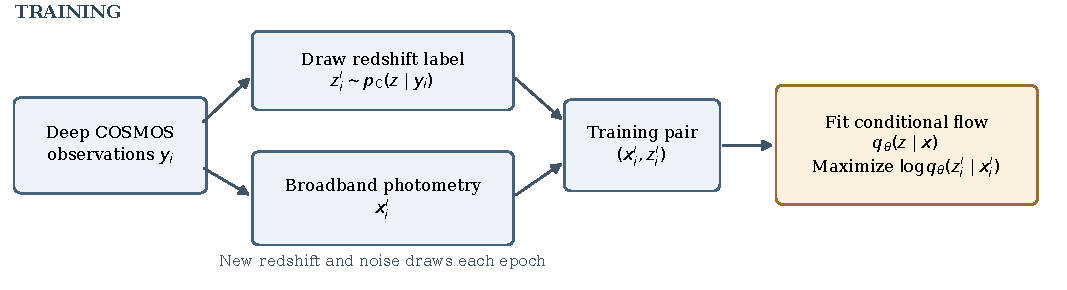
\includegraphics[width=\textwidth]{figures/fig05_bootstrap_workflow.pdf}
\caption{\label{fig:workflow}
Workflow of the bootstrapped flow. For each training galaxy, we independently
draw a redshift from its released COSMOS2020 PDF and a noisy broadband
measurement conditional on its deep observations. We fit the conditional
flow to these pairs, drawing new labels and noise each epoch.
The photometric transfer uses the explicit noise model
in Equation~\ref{eq:kernel}; the input redshift PDFs are not recalibrated.}
\end{figure*}

Let $y$ denote the deep observations, $z$ redshift, and
$x=(\bm f,\bm\sigma)$ the broadband fluxes and uncertainties.
For the selected COSMOS population $S$, we assume $z\perp x\given y,S$.
If the released distribution $p_{\rm C}(z\given y)$ describes the true
conditional redshift distribution, then
\begin{equation}
p(z\given x,S)=\int p_{\rm C}(z\given y)\,p(y\given x,S)\,dy.
\label{eq:target}
\end{equation}
We approximate this integral by sampling redshifts from the released PDFs
and broadband measurements from the noise model $K(x\given y)$ in
Equation~\ref{eq:kernel}. We train a conditional normalizing flow
$q_\theta(z\given x)$ by minimizing
\begin{equation}
\mathcal L(\theta)=-\frac{1}{N}\sum_i
\mathbb E_{\substack{z\sim p_{\rm C}(z\given y_i)\\
                    x\sim K(x\given y_i)}}
\left[\log q_\theta(z\given x)\right].
\label{eq:loss}
\end{equation}
We draw a new redshift and new photometric noise for each galaxy at each
training traversal. These draws are independent conditional on $y_i$.
We normalize the released PDFs over $0\leq z\leq10$, interpolate their
densities linearly between grid points ($\Delta z=0.01$), and sample by
inverting the continuous cumulative distribution. We apply no recalibration
to the input PDFs. We call this estimator the \emph{bootstrapped flow}.

Equation~\ref{eq:loss} fits the conditional distribution defined by the
input PDFs, photometric population, and noise model. It therefore propagates
any errors or prior dependence in those PDFs. We do not divide the labels
by a global $p(z)$: our target is a conditional redshift distribution for
$S$, not a redshift likelihood. Applying the model to another population
requires checking population coverage and selection. This experiment tests
neither the sufficiency assumption nor the correctness of the input PDFs.

The flow uses two conditional rational-quadratic spline transforms, each
with 16 bins, hidden width 64, and two residual blocks, with a standard-normal
base \citep{durkan2019}. We transform redshift as
$t=\{\log[z/(10-z)]+2.2\}/1.1$ and include its Jacobian in the density.
Inputs are six asinh-transformed fluxes with softening $0.02\,\mu$Jy and
six log uncertainties. We estimate feature normalization from the full
photometric training set.

We train with AdamW, learning rate $8\times10^{-4}$, batches of 512,
and gradient clipping at 5. We allow at most 200 epochs and 20,000 steps,
with validation-based learning-rate reduction and early stopping.
The bootstrapped flow uses fixed posterior draws for validation; the
broadband flow uses spectroscopic labels. They train for 20,000 and
7,515 steps, respectively. We use one training seed for each model.
